\documentclass[spanish,12pt,a4paper]{article}
\usepackage[T1]{fontenc}
\usepackage{geometry}
\usepackage{graphicx}
\usepackage{mathtools}
\usepackage{amssymb}
\usepackage{amsthm}
\usepackage{xcolor}
\usepackage{babel}
\usepackage{hyperref}
\usepackage{longtable}
\title{Informe comisión y promoción}
\author{Brayan Romero}
\begin{document}
	
	%
	\begin{center}
		\begin{tabular}{|p{3cm}|p{12cm}|}
			\hline
			\vspace{0.05cm}
			\centering
			
\includegraphics[scale=0.35]{logo.png}
			&
			\begin{center}
				\textbf{GIMNASIO PSICOPEDAGÓGICO SUBA}
				
				\vspace{0.1cm}
				El amor, fuente fundamental para la formación integral
				
				\vspace{0.1cm}
				\textbf{PLAN DE MEJORAMIENTO}
				
				\vspace{0.1cm}
				\textbf{GRADO DÉCIMO}
				
			\end{center}
			\\
			\hline
			
			
		\end{tabular}
		
	\end{center}	
	
	\section*{OBJETIVO:}
	Resolver problemas en los cuales se hace necesaria la utilización de operaciones aritméticas entre números naturales para aplicarlo en contextos reales de su vida cotidiana. 
	
	\section*{PROCEDIMIENTO Y CRONOGRAMA:}
	\begin{enumerate}
		\item Entrega del plan de mejoramiento al padre de familia.
		\item Entrega de los talleres desarrollados al docente de la asignatura, el día \textcolor{red}{14 de mayo de 2024} en físico.
		\item El estudiante debe realizar la sustentación el día \textcolor{red}{14 de mayo de 2024}.
	\end{enumerate}
	
	\section*{OBSERVACIONES:}
	\textbf{Se solicita leer las observaciones y estudiar la actividad antes de comenzar.}
	\begin{itemize}
		\item Si tiene alguna duda sobre los puntos del plan, diríjase al docente para aclararlas, en horas laborales, antes de entregar el plan de mejoramiento, de no hacerlos, no se aceptarán reclamos que estén fuera de los lineamientos ni excusas.
		
		\item Todas las actividades asignadas son de carácter obligatorio, ya que hacen parte de los temas trabajados durante el periodo. Estas deben ser entregadas sin excepción y sustentadas según fecha indicada.
		
		\item La presentación del trabajo completo, en la fecha correspondiente, es indispensable para la evaluación de la misma.
		
		\item La presentación completa del trabajo tendrá un valor del 40\% y su evaluación respectiva 60\%. Toda asignatura recuperada tendrá una nota de Aprobado (DB) (70): Desempeño Básico; y su nota será modificada en el boletín correspondiente al siguiente período.
		
		\item \textbf{Por lo anterior se debe tener en cuenta que el estudiante que no pase la evaluación tampoco pasará la recuperación. Por lo mismo, aquel que no presente alguna actividad tampoco podrá presentar la evaluación.}
		
		\item Los estudiantes deberán asistir a las actividades de recuperación con el uniforme.
		
		\item La actividad debe ser desarrollada en su totalidad por el ESTUDIANTE a mano.
		
		\item La presentación del trabajo se tendrá en cuenta. Trabajos arrugados y hechos a la carrera no serán calificados. \textbf{La caligrafía y ortografía} debe ser digna de un trabajo de recuperación. Se recomienda una excelente presentación de los trabajos con portada y en carpeta que sean dignos de calificación.
		
		\item \textbf{El orden, la actitud y la disciplina al momento de la sustentación también se tendrá en cuenta.}
		
		\item \textbf{Respuesta copiada textual de internet, será anulada.}
	\end{itemize}
	
	\vspace{0.5cm}
	\section*{PLAN DE MEJORAMIENTO}
	\subsection*{Grado Décimo}
	
	A continuación se presenta la lista de desempeños a evaluar en el plan de mejoramiento, cada estudiante realizará los puntos según el desempeño perdido. El estudiante que tenga la asignatura reprobada deberá realizar el plan de mejoramiento en su totalidad.\\
	
	
	\textbf{D1:} Distingue entre las diferentes unidades de medida que se pueden usar en los ángulos.
	
	\textbf{D2:} Reconoce las graficas de seno y coseno y las dibuja a partir de la circunferencia unitaria.
	
	\textbf{D3:} Reconoce las graficas de las funciones trigonométricas, seno, coseno, tangente, cotangente, secante y cosecante.
	
	\textbf{D4:} Reconoce los ángulos notables de las funciones trigonométricas de 0° a 90°.
	
	\textbf{D5:} Reconoce los ángulos notables de las funciones trigonométricas de 0° a 360°.
	
	\textbf{D6:} Reconoce la gráfica de las funciones trigonométricas a partir de la transformación de funciones trigonométricas más sencillas.
	
	\textbf{D7:} Convierte de grados decimales a radianes y de grados decimales a grados minutos y segundos.
	
	\textbf{D8:} Encuentra la grafica de funciones trigonométricas a partir de las transformaciones de funciones.
	
	
	%---------------------------------------------------
	%---------------------------------------------------
	%---------------------------------------------------
	\vspace{1cm}
	
	\begin{itemize}
		\item \textbf{Desempeños trigonometría aplicada}
		
		\begin{figure}[h]
			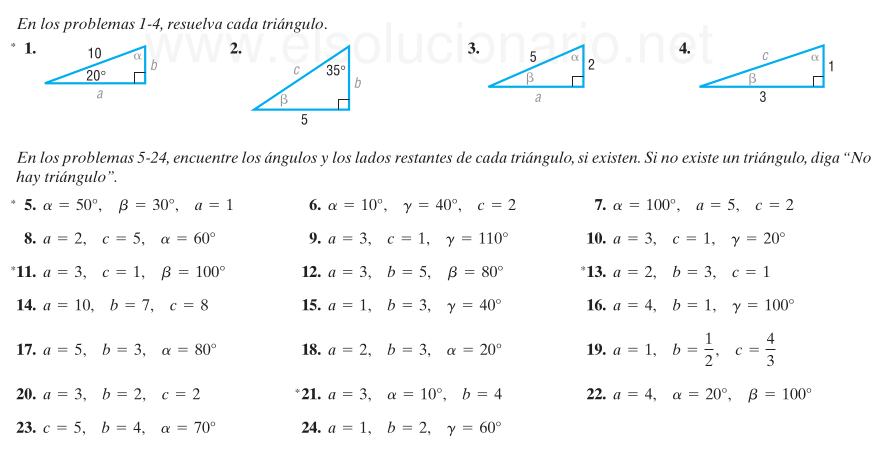
\includegraphics[scale=0.5]{triangulo_rectangulo.png}
		\end{figure}
		\newpage
		\item \textbf{Desempeños trigonometría analítica}
		\begin{figure}[h]
			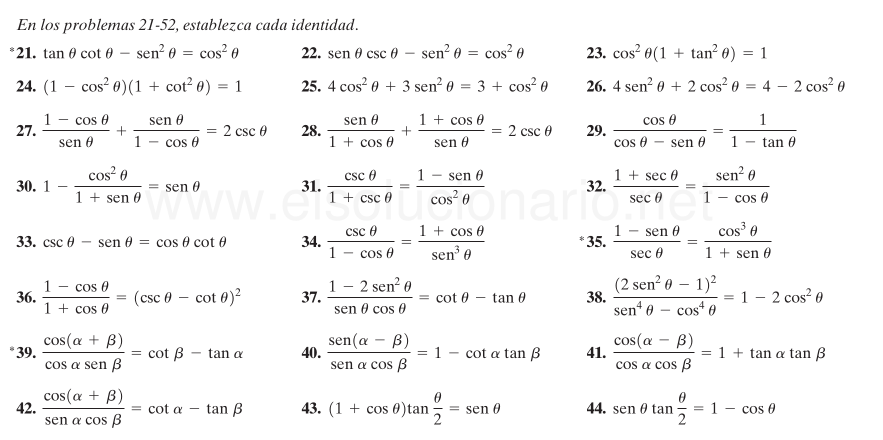
\includegraphics[scale=0.5]{identidades.png}
		\end{figure}
	\end{itemize}
	
	
\end{document}